\documentclass[12pt]{article}

\usepackage{amsmath,amsthm,amsfonts,amssymb,amsxtra}
\usepackage{pgf,tikz}
\usetikzlibrary{arrows}
\renewcommand{\theenumi}{(\alph{enumi})} 
\renewcommand{\labelenumi}{\theenumi}

\pagestyle{empty}
\setlength{\textwidth}{7in}
\setlength{\oddsidemargin}{-0.5in}
\setlength{\topmargin}{-1.0in}
\setlength{\textheight}{9.5in}

\theoremstyle{definition}
\newtheorem{problem}{Problem}

\begin{document}

\noindent{\large\bf MATH 241}\hfill{\large\bf Exam \#2}\hfill{\large\bf
  Spring 2018}\hfill{\large\bf Page 1/6}\hrule

\bigskip
\begin{center}
  \begin{tabular}{|ll|}
    \hline & \cr
    {\bf Name: } & \makebox[12cm]{\hrulefill}\cr & \cr
    {\bf 4-digit code:} & \makebox[12cm]{\hrulefill}\cr & \cr
    \hline
  \end{tabular}
\end{center}
\begin{itemize}
\item Write your name and your VIP ID in the space provided above.
\item The test has six (6) pages, including this one, and scratch page at the end.
\item Enter your answer in the box(es) provided.
\item You must show sufficient work to justify all answers unless
  otherwise stated in the problem.  Correct answers with inconsistent
  work may not be given credit.
\item Credit for each problem is given in parentheses at the right of
  the problem number.
\end{itemize}
\hrule

\begin{center}
  \begin{tabular}{|c|c|c|}
    \hline
    &&\cr
    {\large\bf Page} & {\large\bf Max.~points} & {\large\bf Your points} \cr
    &&\cr
    \hline
    &&\cr
    {\Large 2} & \Large 20 & \cr
    &&\cr
    \hline
    &&\cr
    {\Large 3} & \Large 30 & \cr
    &&\cr
    \hline
    &&\cr
    {\Large 4} & \Large 30 & \cr
    &&\cr
    \hline
    &&\cr
    {\Large 5} & \Large 20 & \cr
    &&\cr
    \hline\hline
    &&\cr
    {\large\bf Total} & \Large 100 & \cr
    &&\cr
    \hline
  \end{tabular}
\end{center}
\newpage

%%%%%%%%%%%%%%%%%%%%%%%%%%%%%%%%%%%%% Page 2
\noindent{\large\bf MATH 241}\hfill{\large\bf Exam \#2}\hfill{\large\bf
  Spring 2018}\hfill{\large\bf Page 2/6}\hrule

\bigskip
\begin{problem}[10 pts] 
Find (and sketch) the domain of $f(x,y)=\dfrac{\sqrt{4-x^2}}{y^2+3}$

\begin{tikzpicture}
\draw [white] (-3.5,-3.5) rectangle (3.5,3.5);
\draw [<->, ultra thick] (-3.5,0) -- (3.5,0);
\draw [<->, ultra thick] (0,-3.5) -- (0,3.5);
\draw[step=0.5,black,thin] (-3.25, -3.25) grid (3.25, 3.25);
\draw (4.5, -3.5) -- (4.5, 3.5);
\draw (6.5,3) node {Show work here:};
\end{tikzpicture}
\begin{flushright}
  \begin{tikzpicture}
    \draw (-8.0cm,2.1cm) node {domain:};
    \draw (-7cm,1.4cm) rectangle (5cm,2.8cm);
  \end{tikzpicture}
\end{flushright}
\end{problem}
\hrule
\begin{problem}[10 pts---5 points each part]
For the function $f(x,y) = \sqrt{y-x^2+x}$.
\begin{enumerate}
  \item Sketch the level lines $f(x,y)=k$ for $k=-1,0,1,2$ \newline \noindent(whenever the equations make sense)
  \item Use the previous information to compute the range of the function $f$.
\end{enumerate}

\begin{tikzpicture}
\draw [white] (-3.5,-3.5) rectangle (3.5,3.5);
\draw [<->, ultra thick] (-3.5,0) -- (3.5,0);
\draw [<->, ultra thick] (0,-3.5) -- (0,3.5);
\draw[step=0.5,black,thin] (-3.25, -3.25) grid (3.25, 3.25);
\draw (4.5, -3.5) -- (4.5, 3.5);
\draw (6.5, 3) node {Show work here:};
\end{tikzpicture}
\begin{flushright}
  \begin{tikzpicture}
    \draw (-1.0cm,2.1cm) node {range:};
    \draw (-0cm,1.4cm) rectangle (5cm,2.8cm);
  \end{tikzpicture}
\end{flushright}
\end{problem}
\newpage

%%%%%%%%%%%%%%%%%%%%%%%%%%%%%%%%%%%%% Page 3
\noindent{\large\bf MATH 241}\hfill{\large\bf Exam \#2}\hfill{\large\bf
  Spring 2018}\hfill{\large\bf Page 3/6}\hrule

\bigskip
\begin{problem}[10 pts] 
Find the tangent plane to the elliptic paraboloid
$z=f(x,y)=2x^2+y^2$ at the point $(1,1,3)$.
\vspace{5cm}
\begin{flushright}
  \begin{tikzpicture}
    \draw (0cm,-0.2cm) rectangle (5cm,1.2cm);
  \end{tikzpicture}
\end{flushright}
\end{problem}
\hrule
\begin{problem}[10 pts] Find the partial derivatives $\frac{\partial f}{\partial x}$ and $\frac{\partial f}{\partial y}$ of the function $f(x,y) = \dfrac{xy^2}{y+2x}$.
\vspace{4.5cm}
\begin{flushright}
  \begin{tikzpicture}
    \draw (-11.8cm, 0.5cm) node {$\dfrac{\partial f}{\partial x} = $};
    \draw (-11cm,-0.2cm) rectangle (-4cm,1.2cm);
    \draw (-2.8cm, 0.5cm) node {$\dfrac{\partial f}{\partial y} = $};
    \draw (-2cm, -0.2cm) rectangle (5cm,1.2cm);
  \end{tikzpicture}
\end{flushright}
\end{problem}
\hrule
\begin{problem}[10 pts]
Compute the directional derivative $D_{\boldsymbol{v}}f(0,\pi)$ for the function $f(x,y) = e^x \cos(xy^2-2y)$ and the direction of the vector $\boldsymbol{v} = \boldsymbol{i} + \boldsymbol{j}$.
\vspace{5cm}
\begin{flushright}
  \begin{tikzpicture}
    \draw (-1.2cm,0.5cm) node {$D_{\boldsymbol{v}} f(0,\pi) = $};
    \draw (0cm,-0.2cm) rectangle (5cm,1.2cm);
  \end{tikzpicture}
\end{flushright}
\end{problem}
\newpage

%%%%%%%%%%%%%%%%%%%%%%%%%%%%%%%%%%%%% Page 4
\noindent{\large\bf MATH 241}\hfill{\large\bf Exam \#2}\hfill{\large\bf
  Spring 2018}\hfill{\large\bf Page 4/6}\hrule

\bigskip
\begin{problem}[15 pts---5 pts each box] 
Find the local maxima, minima and saddle points
of $f(x)=x^4+y^4-4xy+1.$
\vspace{5cm}
\begin{center}
  \begin{tabular}{ccc}
  \begin{tikzpicture}
    \draw (0cm,-0.2cm) rectangle (5cm,1.2cm);
    \draw (0.5cm,1cm) node[scale=0.8]{max};
  \end{tikzpicture} &
  \begin{tikzpicture}
    \draw (0cm,-0.2cm) rectangle (5cm,1.2cm);
    \draw (0.5cm,1cm) node[scale=0.8]{min};
  \end{tikzpicture} &
  \begin{tikzpicture}
    \draw (0cm,-0.2cm) rectangle (5cm,1.2cm);
    \draw (1cm,1cm) node[scale=0.8]{saddle pts.};
  \end{tikzpicture}
  \end{tabular}
\end{center}
\end{problem}
\hrule

\begin{problem}[15 pts]
Find the absolute maximum and minimum values of the function $f(x,y) = 4x+6y-x^2-y^2+7$ on the set $D = \big\{ (x,y) : 0 \leq x \leq 4, 0 \leq y \leq 5 \big\}$.  Make sure to sketch the set $D$ and indicate the different borders.
\end{problem}
\newpage

%%%%%%%%%%%%%%%%%%%%%%%%%%%%%%%%%%%%% Page 5
\noindent{\large\bf MATH 241}\hfill{\large\bf Exam \#2}\hfill{\large\bf
  Spring 2018}\hfill{\large\bf Page 5/6}\hrule

\bigskip
\begin{problem}[20 pts---5 pts each]
Consider the function $z=f(x,y)=e^{xy}$
\begin{enumerate}
  \item What is the \emph{maximum value} of any of the directional derivatives of $f$ at the point $(2,0)$?
  \vspace{2.5cm}
  \begin{flushright}
  \begin{tikzpicture}
    \draw (-4cm,0.5cm) node {Value of maximum directional derivative: };
    \draw (0cm,-0.2cm) rectangle (5cm,1.2cm);
  \end{tikzpicture}
\end{flushright}
  \item Are there any directions $\boldsymbol{u}$ for which the directional derivative $D_{\boldsymbol{u}}f(2,0)=0$?  If so, find at least one such direction.
  \vspace{2.5cm}
  \begin{flushright}
  \begin{tikzpicture}
    \draw (-0.5cm, 0.5cm) node {$\boldsymbol{u} = $};
    \draw (0cm,-0.2cm) rectangle (5cm,1.2cm);
  \end{tikzpicture}
\end{flushright}
  \item Are there any directions $\boldsymbol{v}$ for which the directional derivative $D_{\boldsymbol{v}}f(2,0)=-1$?  If so, find at least one such direction.
  \vspace{2.5cm}
  \begin{flushright}
  \begin{tikzpicture}
    \draw (-0.5cm, 0.5cm) node {$\boldsymbol{v} = $};
    \draw (0cm,-0.2cm) rectangle (5cm,1.2cm);
  \end{tikzpicture}
\end{flushright}
  \item Are there any directions $\boldsymbol{w}$ for which the directional derivative $D_{\boldsymbol{w}}f(2,0)=-4$?  If so, find at least one such direction.
  \vspace{2.5cm}
  \begin{flushright}
  \begin{tikzpicture}
    \draw (-0.5cm, 0.5cm) node {$\boldsymbol{w} = $};
    \draw (0cm,-0.2cm) rectangle (5cm,1.2cm);
  \end{tikzpicture}
\end{flushright}
\end{enumerate}
\end{problem}
\newpage

%%%%%%%%%%%%%%%%%%%%%%%%%%%%%%%%%%%%% Page 6
\noindent{\large\bf MATH 241}\hfill{\large\bf Exam \#2}\hfill{\large\bf
  Spring 2018}\hfill{\large\bf Page 6/6}\hrule

\end{document}
